% Implementation, integration and test plan, to be included in dd.tex

\section{Implementation, integration and test plan}
\label{sect:iit}
This section reports the guidelines to implement and test the CLup application. The chosen approach consists in a bottom-up development based on the dependency graph identified in Figure \ref{dep}.

\subsection{Implementation}
The chosen order of implementation, based on the highlighted dependencies and aimed at obtaining core functionalities as soon as possible is the following:
\begin{itemize}[itemsep=-1mm, topsep=-1mm]
	\item Data Access Module
	\item Maps Adapter
	\item SM Account Manager Module
	\item eC Account Manager Module
	\item Queue Manager Module
	\item Visit Manager Module
	\item Access Creation Module
	\item Store Info Manager Module
	\item Store Statistics
	\item Customer Statistics
	\item Store Recommender Module
	\item Access Request Module
	\item Notification Module
	\item Requests Manager Module
	\item Subscription Module
\end{itemize}\vspace{.5\baselineskip} 

If the team is able to handle a good level of parallelization, Figure \ref{deptime} shows a suggestion of steps aimed at minimizing the overall development time; each module's length is dimensioned based on its expected implementation difficulty, and the critical path (that needs not to be delayed in order to meet potential deadlines) is highlighted in red. The graph is also useful for determining which elements can be delayed without impacting the total development time.

\begin{landscape}
	\begin{figure}[p]
		\centering	
		\includegraphics[width=\linewidth] {iit/dependency_graph}
		\caption{Dependency graph}
		\label{dep} 
	\end{figure}

	\begin{figure}[p]
		\centering	
		\includegraphics[width=\linewidth] {iit/dependency_time}
		\caption{Dependency graph with expected time and critical path highlighted}
		\label{deptime} 
	\end{figure}
\end{landscape}

\subsection{Integration and Testing}
\subsubsection{Unit testing}
The unit test can be performed as soon as a component has been developed, or even during its realization to better check its conformity to requirements. Having chosen a bottom-up approach, only Drivers are needed in order to correctly perform unit tests.

% Integration strategy section, to be included in iit.tex

\subsubsection{Integration strategy}
The implementation order has been developed considering the possibility to immediately integrate components and test their interactions; this way development time can be optimized even more and errors can be found as early as possible. The integration strategy is shown in the following figures.

\begin{figure}[h]
	\begin{subfigure}{.42\textwidth}
		\centering
		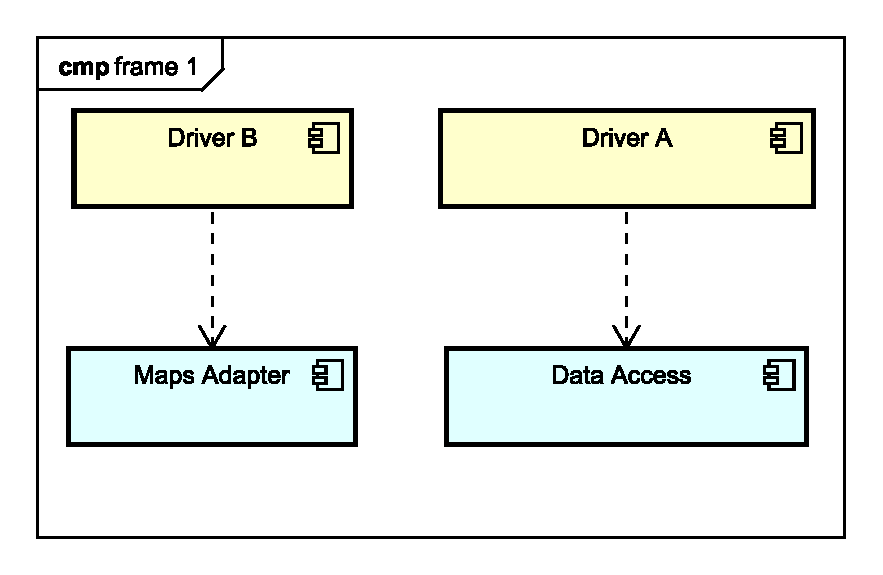
\includegraphics[width=\linewidth]{iit/frame_1}
		\caption{First components with their drivers}
		\label{frame_1}
	\end{subfigure}
	\begin{subfigure}{.58\textwidth}
		\centering
		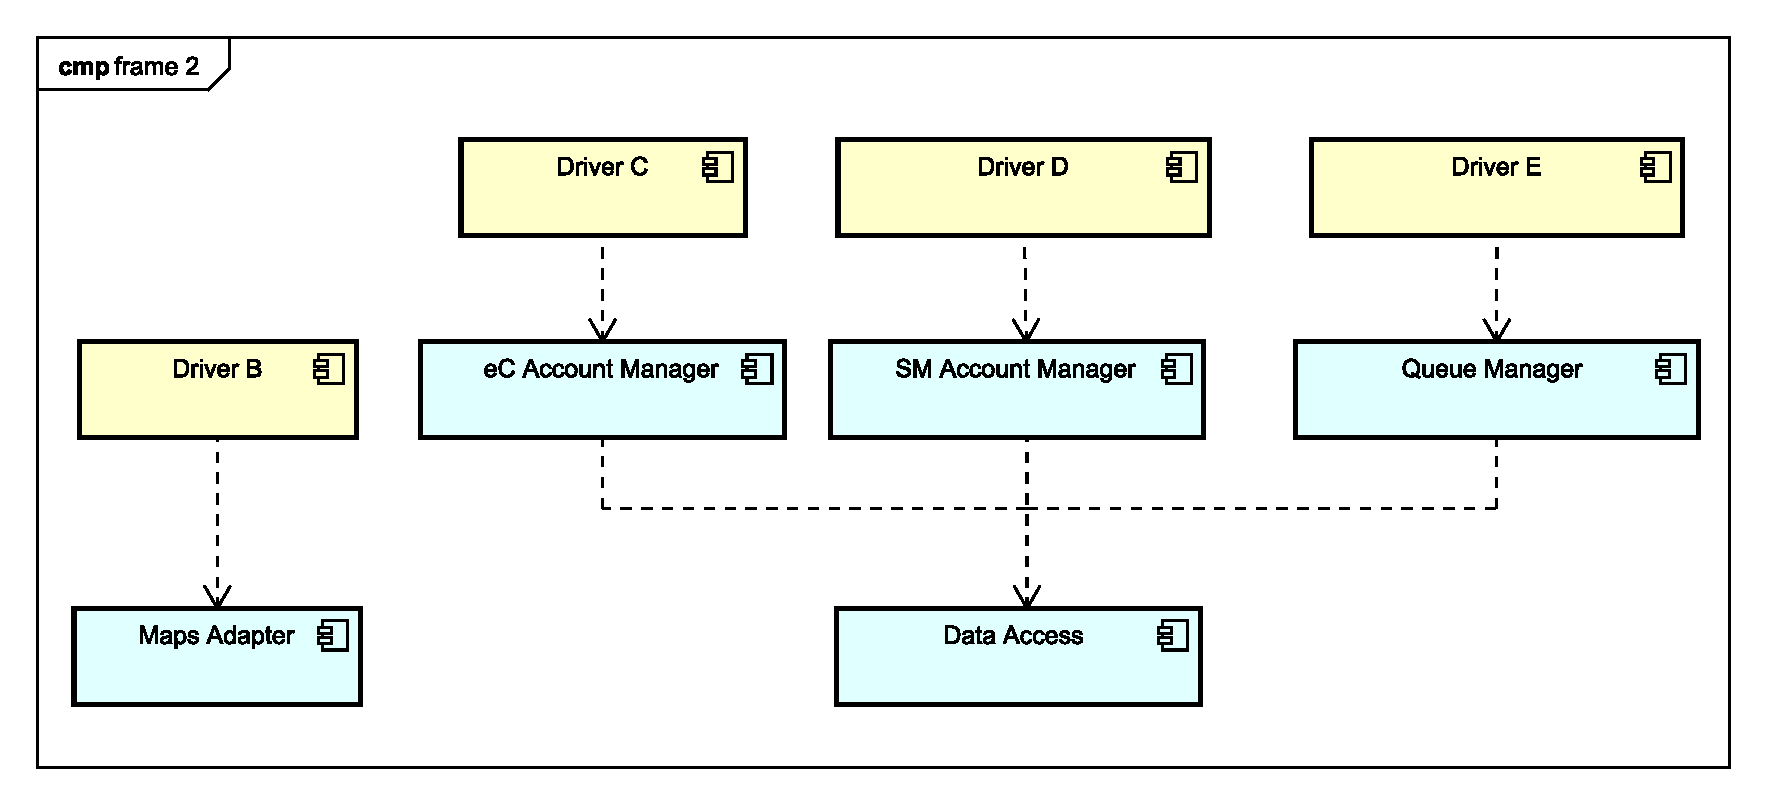
\includegraphics[width=\linewidth]{iit/frame_2}
		\caption{Adding some modules that use function provided by the Data Access and their drivers}
		\label{frame_2}
	\end{subfigure}
\end{figure}

\begin{figure}[h]
	\centering	
	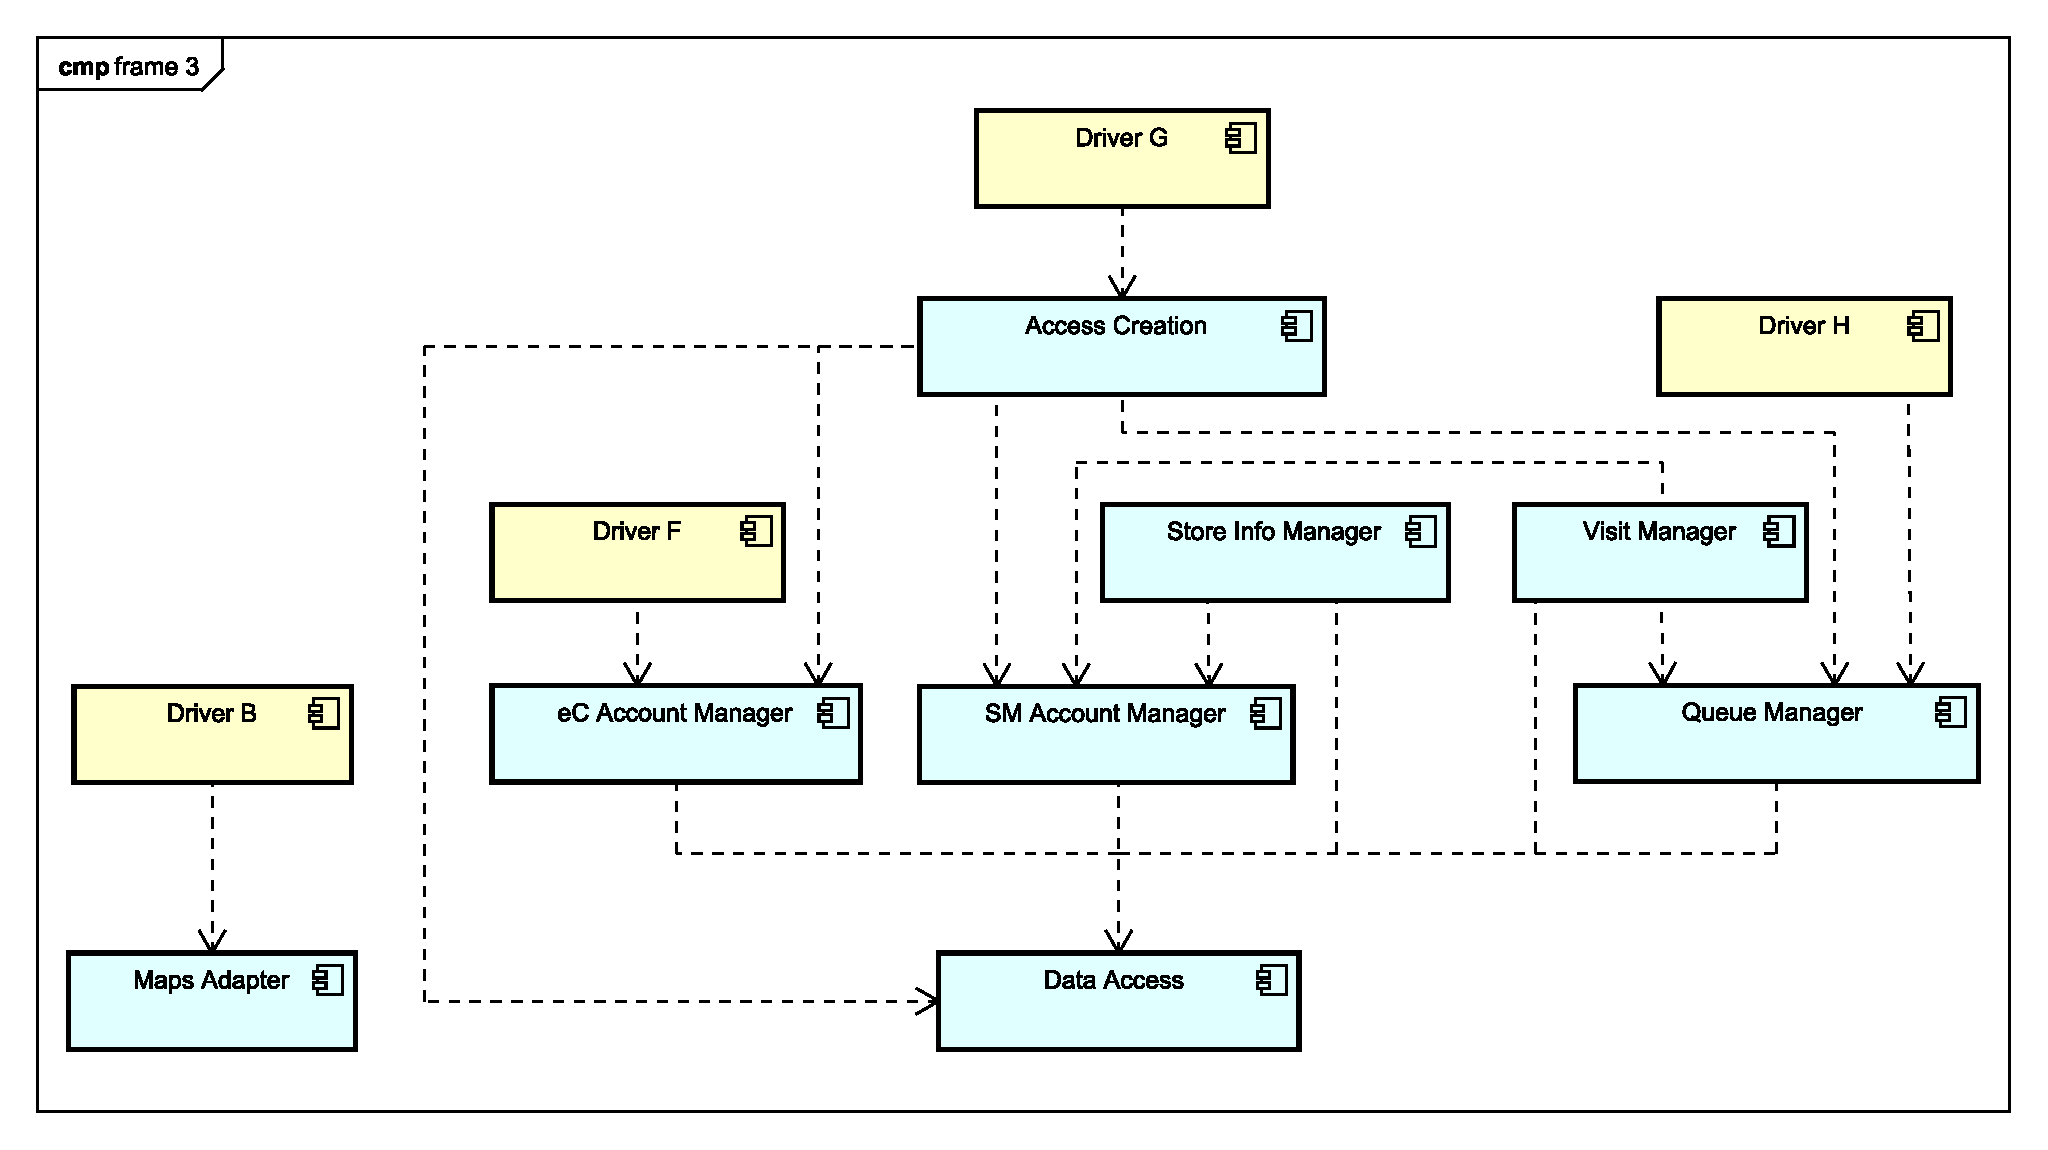
\includegraphics[width=\linewidth] {iit/frame_3}
	\caption{Realization of Access Creation, Store Info Manager, and Visit Modules}
	\label{frame_3} 
\end{figure}

\begin{figure}[p]
	\centering	
	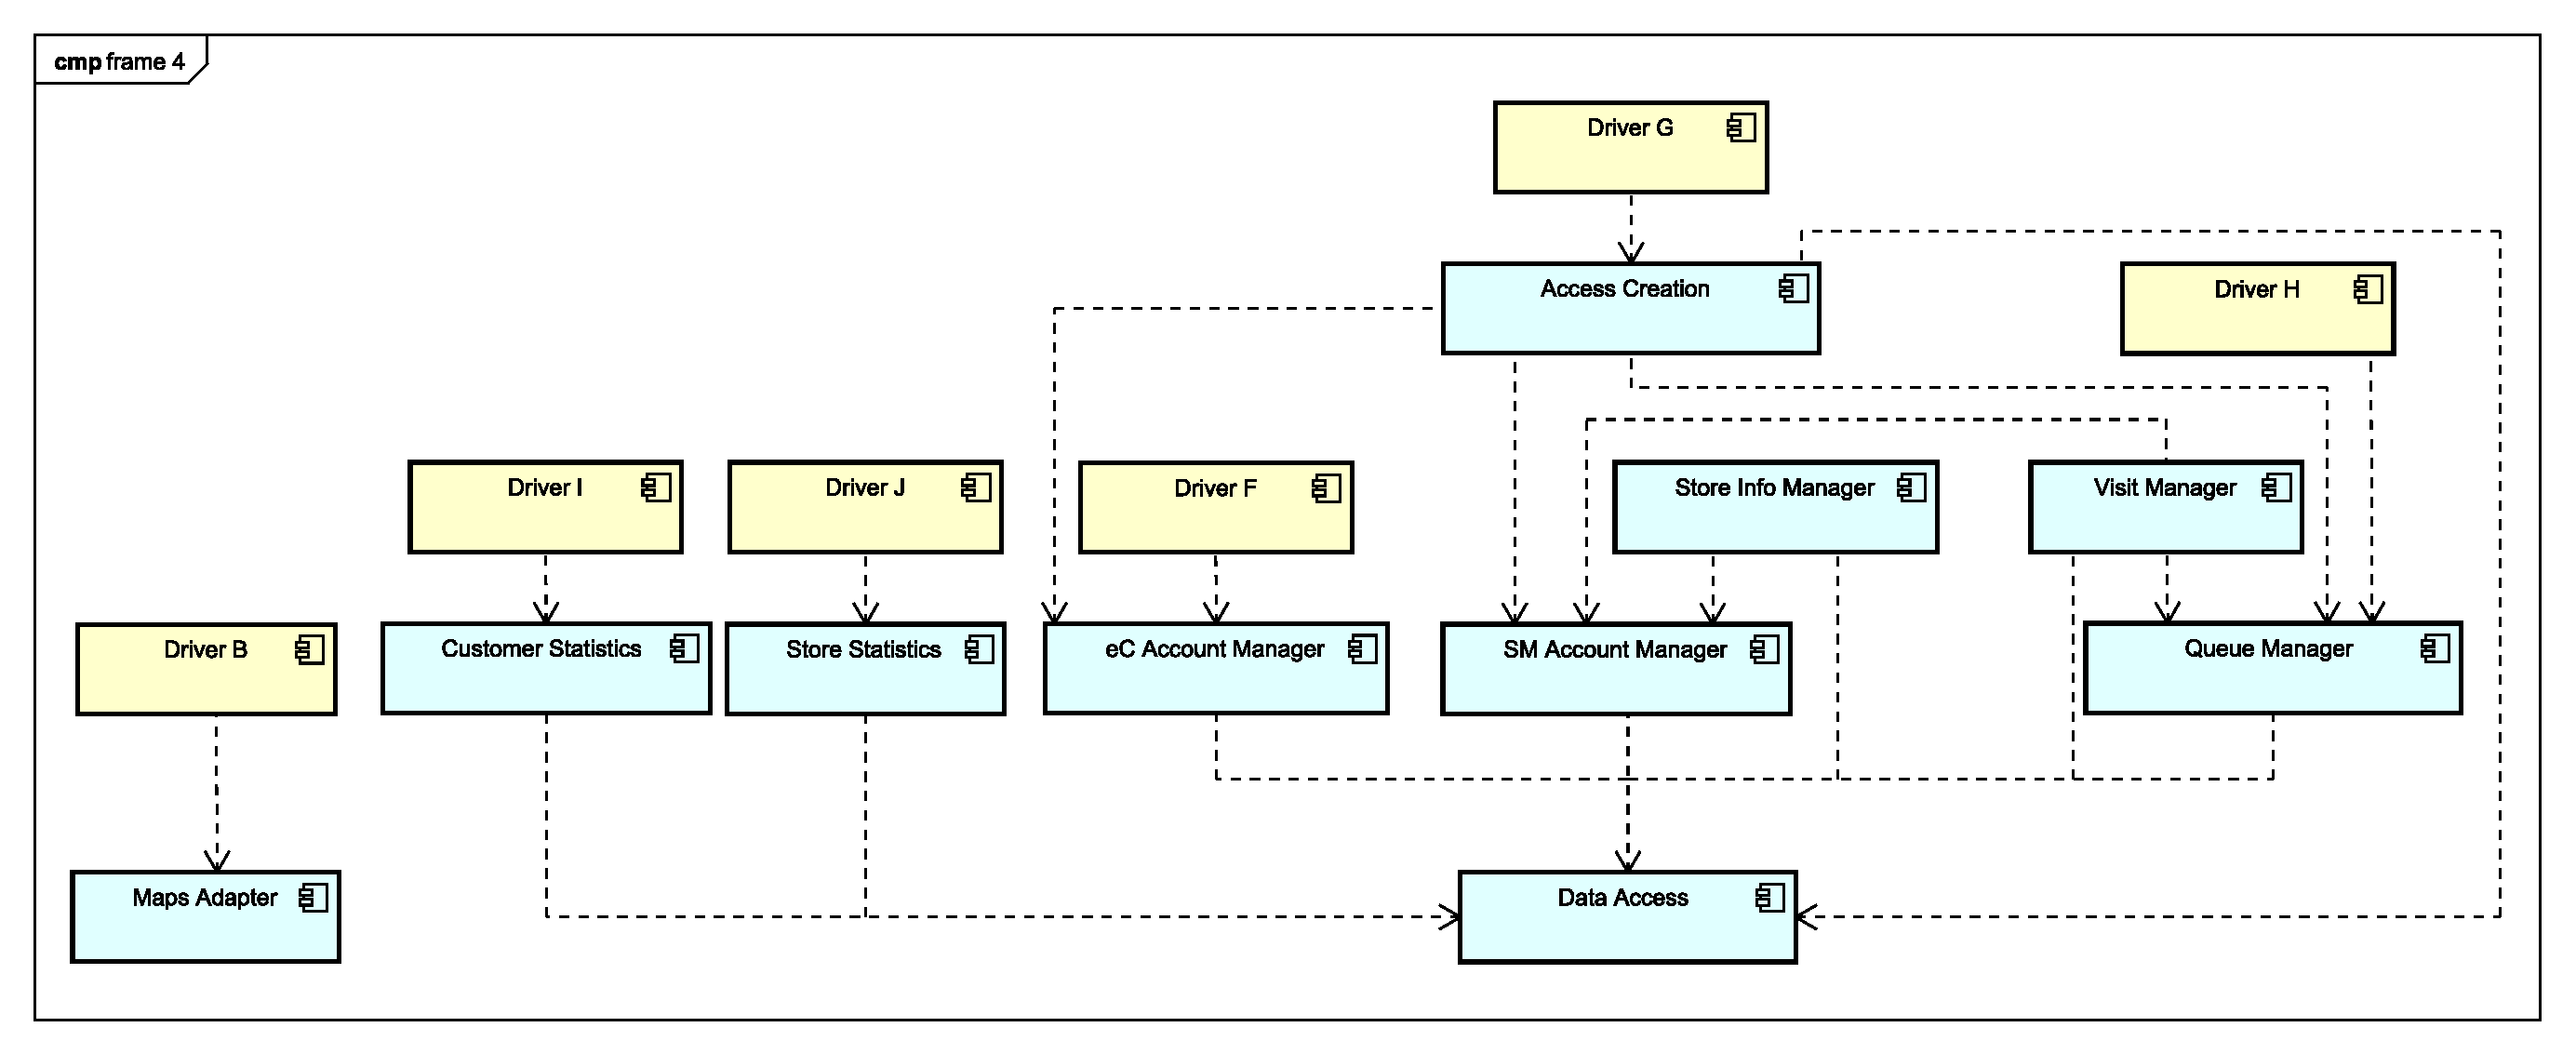
\includegraphics[width=\linewidth] {iit/frame_4}
	\caption{Implementation and integration of Statistics and Store Info Manager Modules}
	\label{frame_4} 

	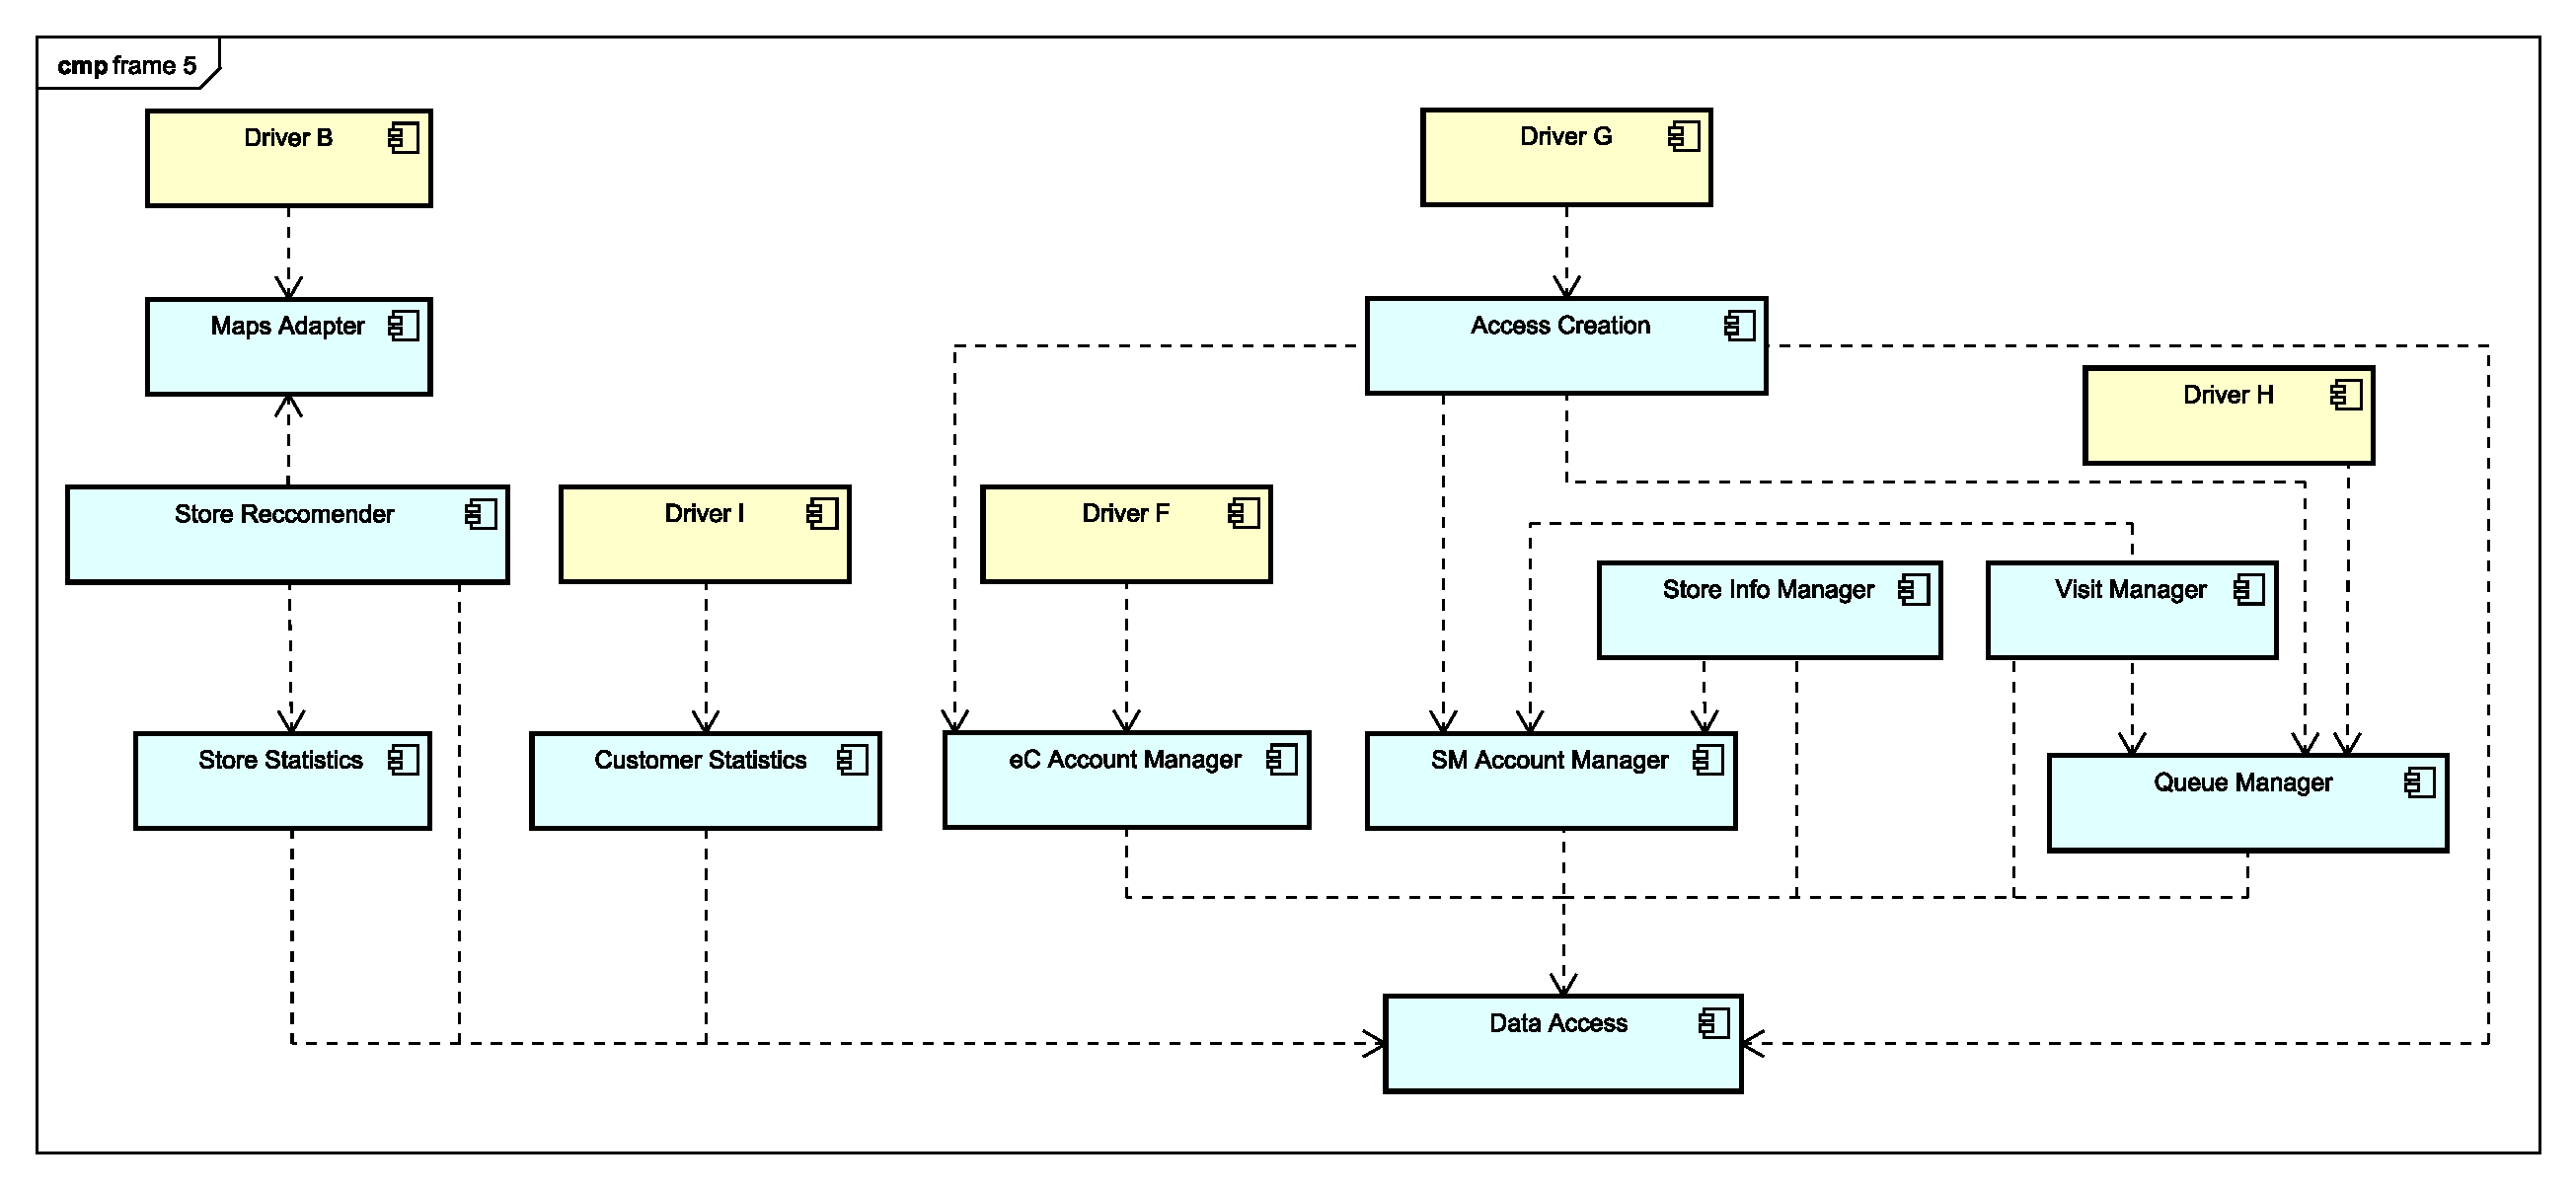
\includegraphics[width=\linewidth] {iit/frame_5}
	\caption{Adding the Store Recommender Module and integrating it with its dependencies}
	\label{frame_5} 

	\centering	
	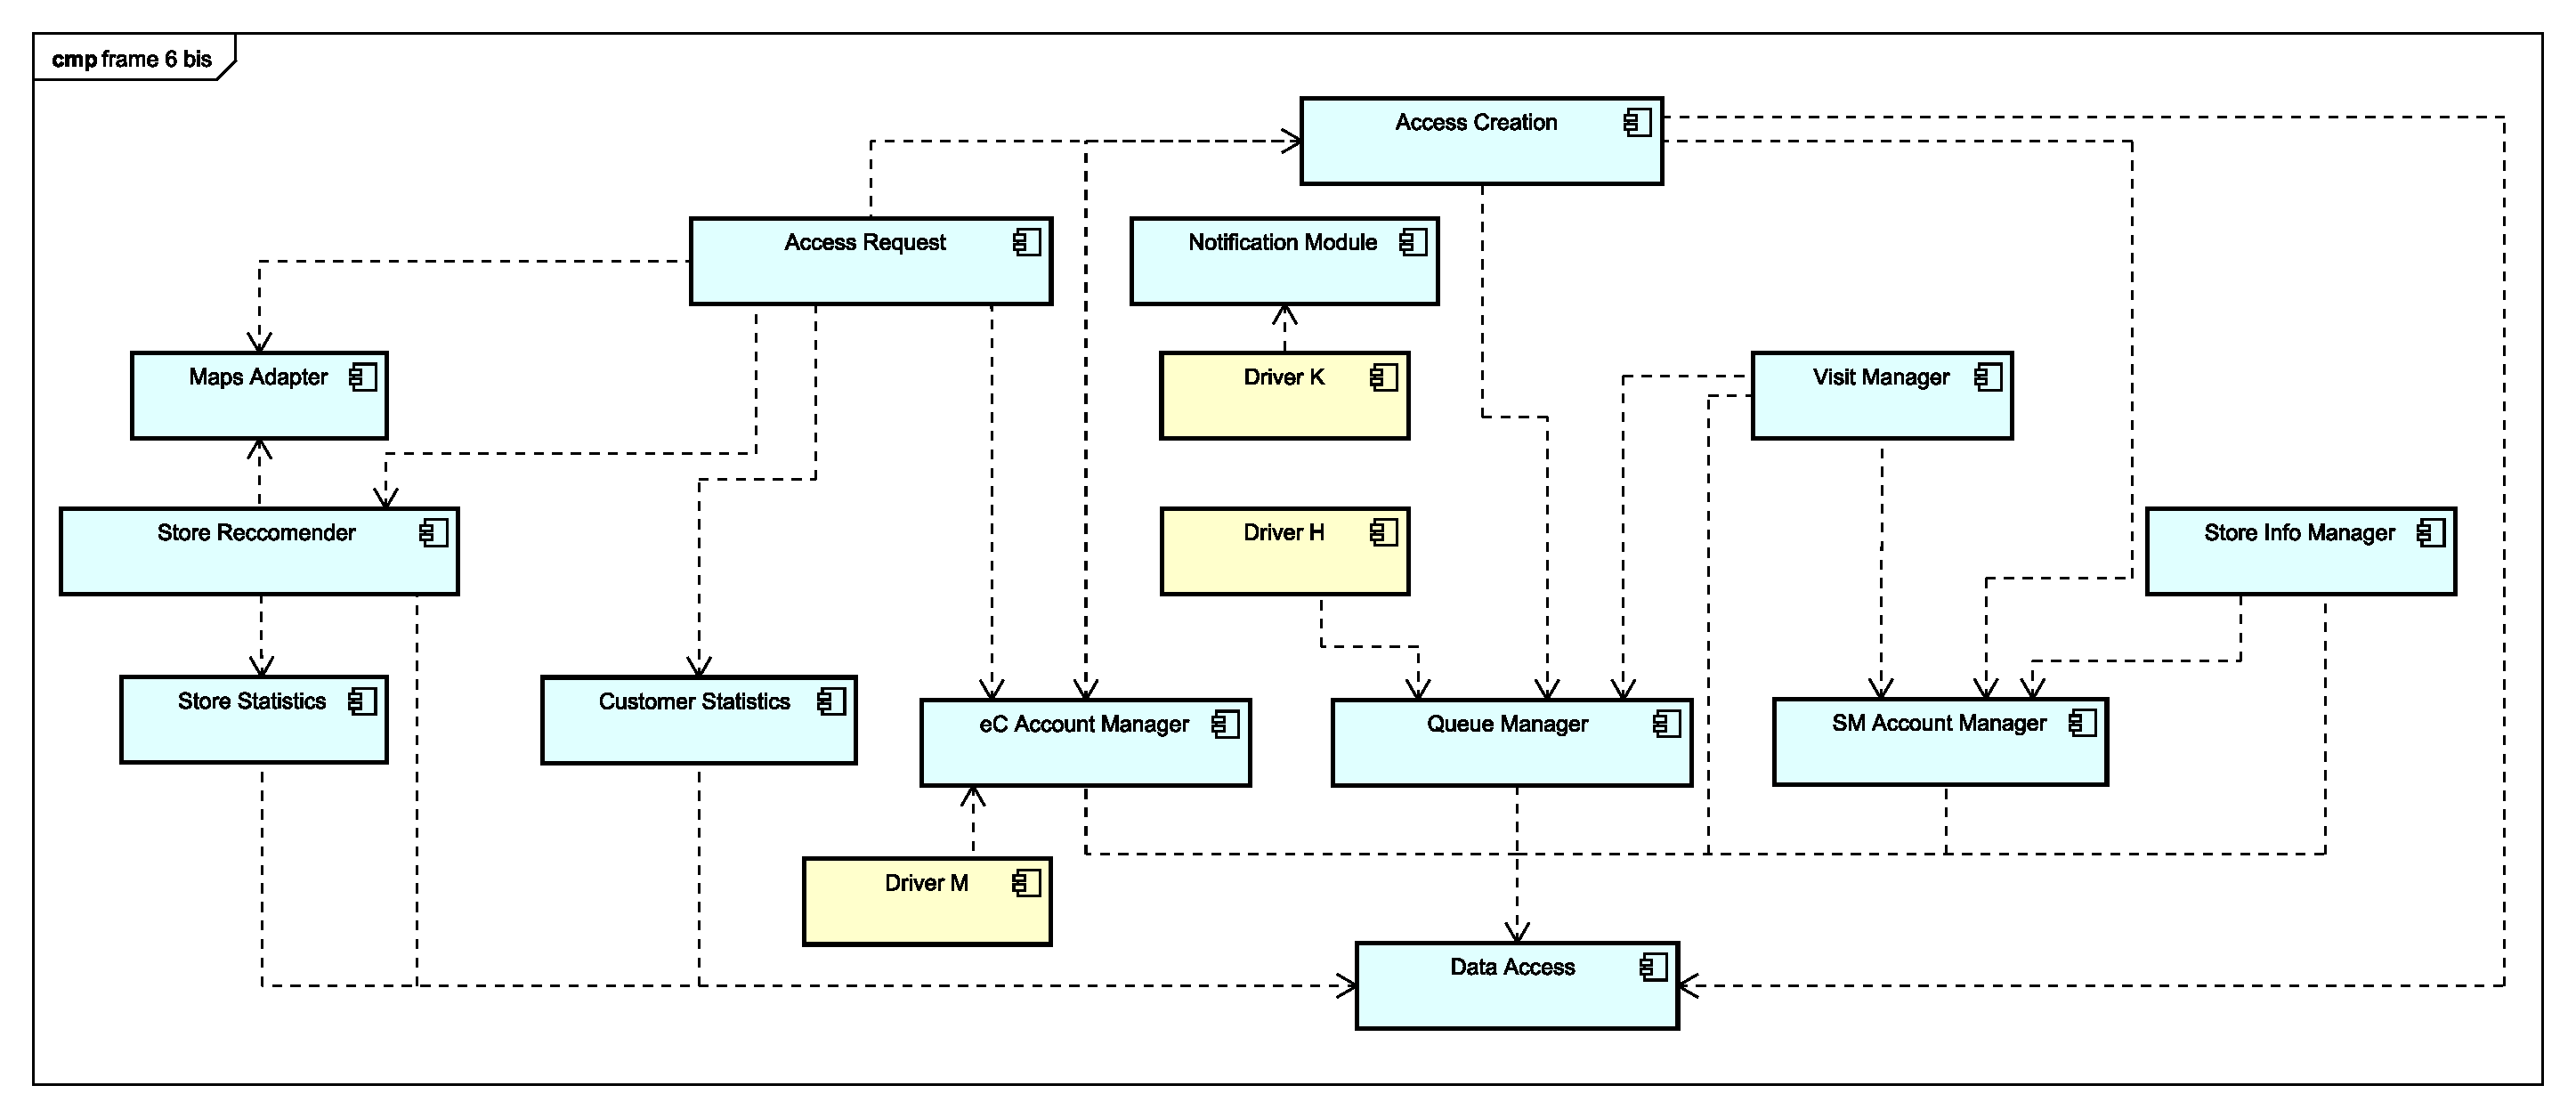
\includegraphics[width=\linewidth] {iit/frame_6}
	\caption{Integration of Access Request and Notification Modules}
	\label{frame_6} 
\end{figure}

\begin{figure}[h]
	\centering	
	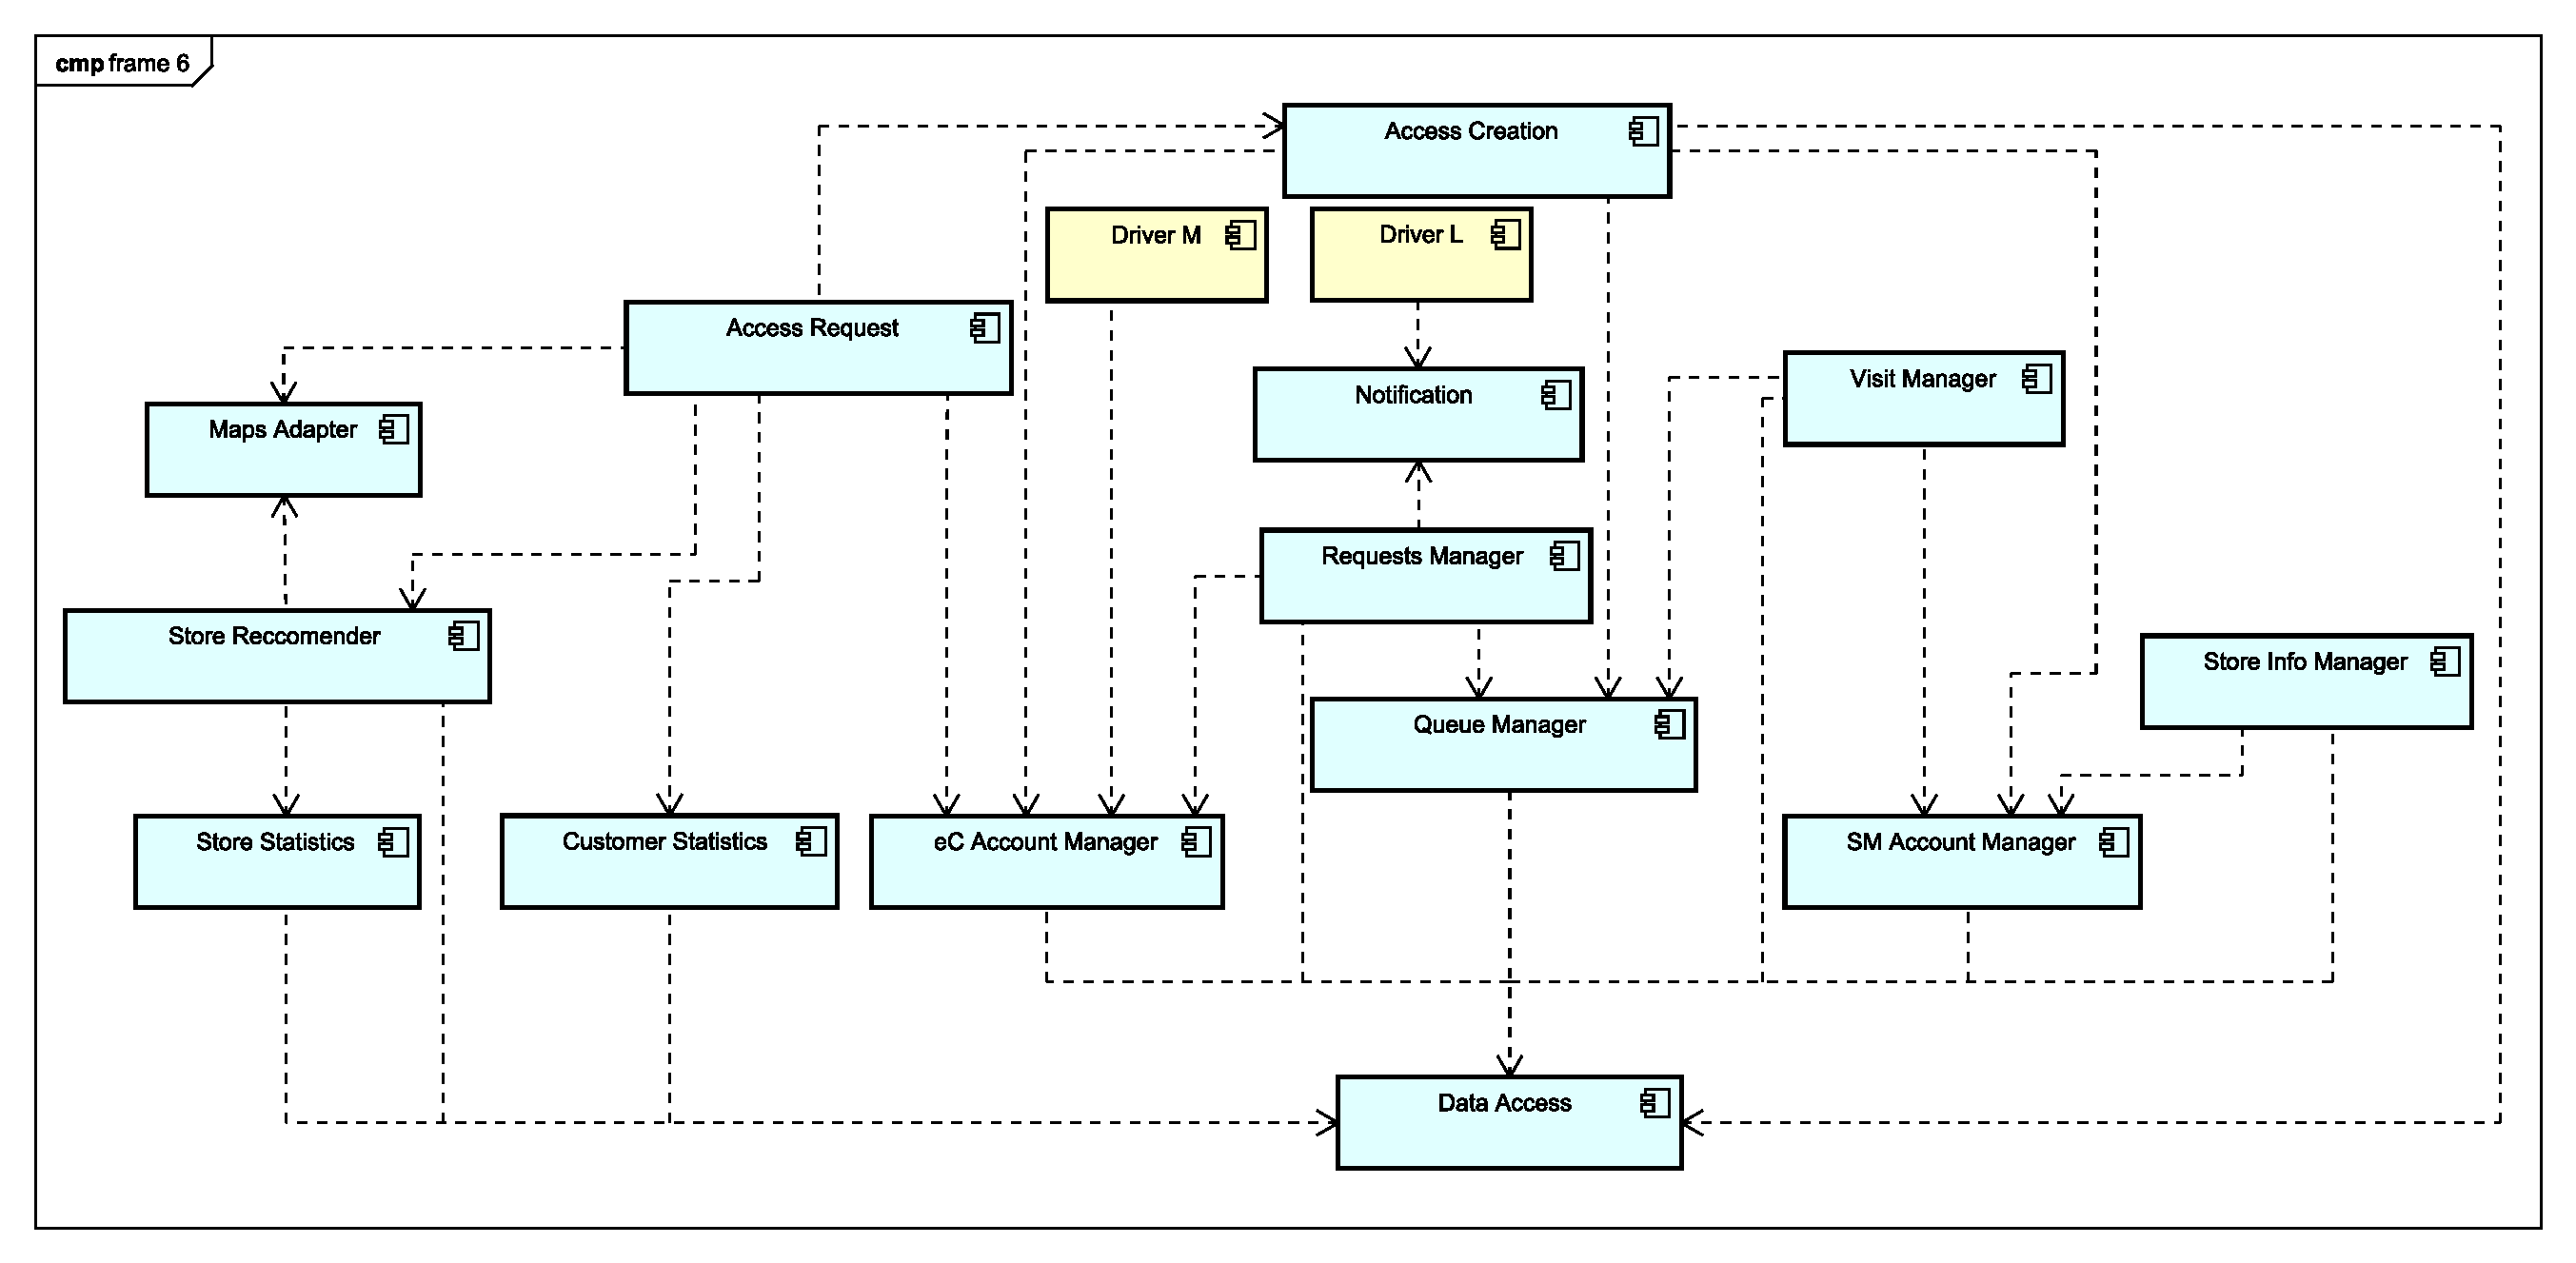
\includegraphics[width=\linewidth] {iit/frame_7}
	\caption{Addition of the Requests Manager Module}
	\label{frame_7} 
\end{figure}

\begin{figure}[h]
	\centering	
	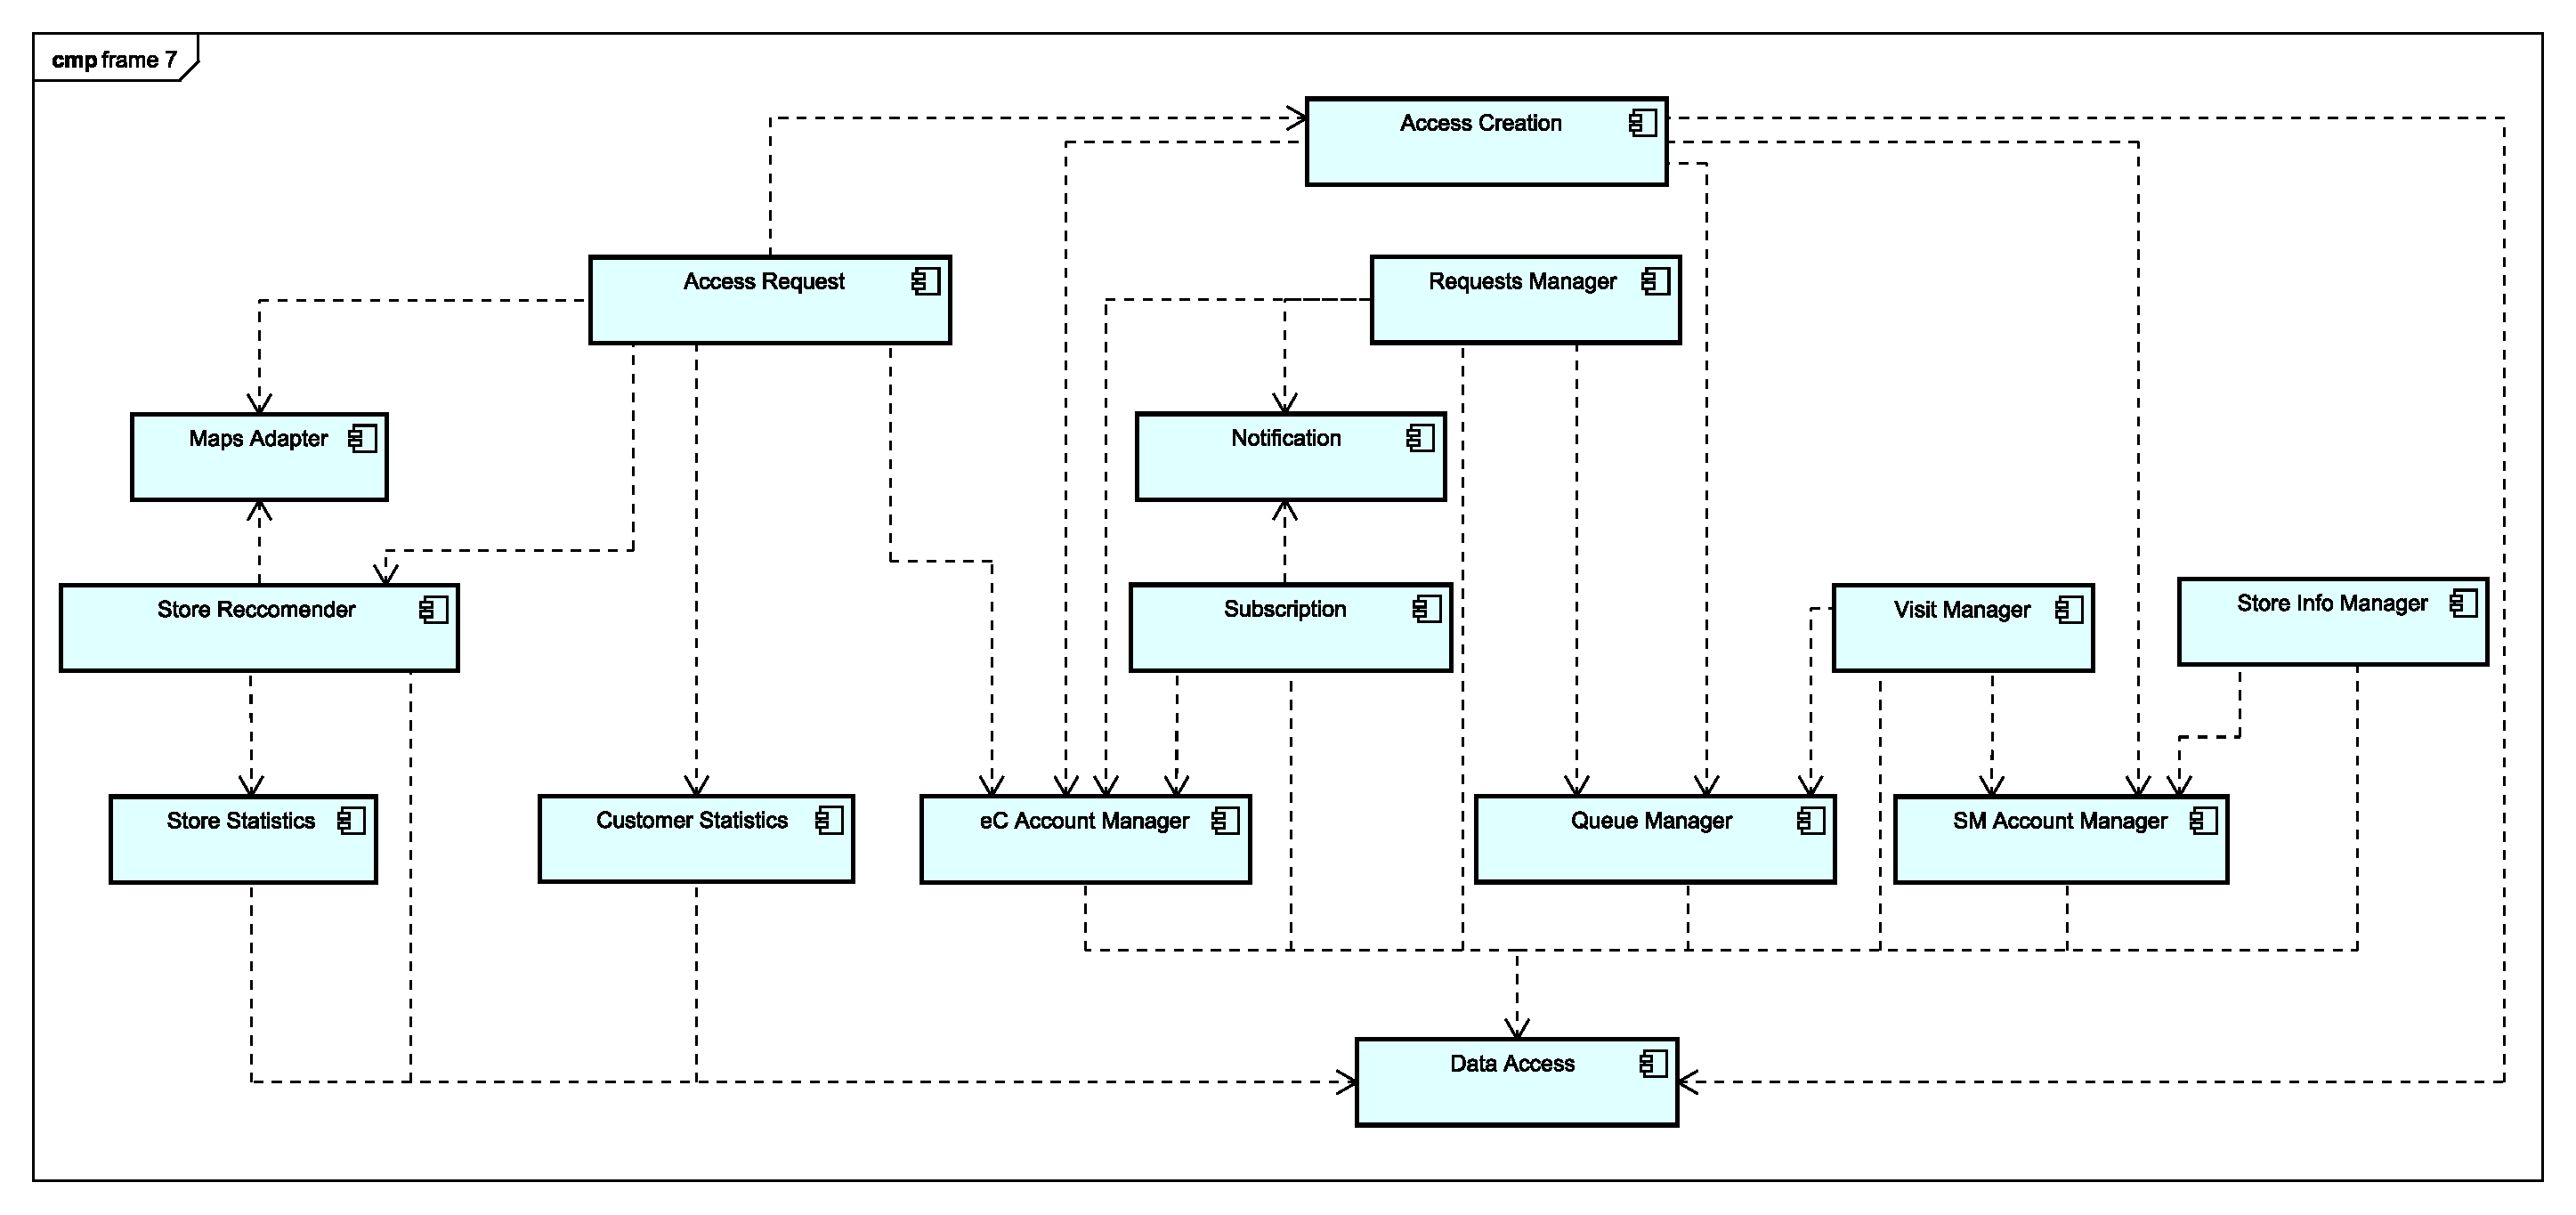
\includegraphics[width=\linewidth] {iit/frame_8}
	\caption{Final module integration with the previously missing Subscription Module}
	\label{frame_8} 
\end{figure}

\clearpage

\subsection{System Testing}
Once all the modules have been integrated, the system as whole should be tested for requirements satisfaction, both functional and non-functional.

\paragraph{Performance Testing}
Checking if the performance constraints defined in the RASD\textsuperscript{\cite{rasdperf}} are met is an important phase when testing the system as a whole. Moreover, it can help with the optimization of algorithms and queries (if helpful) and the identification of bottlenecks.

\paragraph{Load Testing}
This test should check that the system can handle the load defined in the previous document\textsuperscript{\cite{rasdperf}} and is fundamental to expose potential memory occupancy issues.

\paragraph{Stress Testing}
This final test type should test the ability of the system to handle failures and recover from them. 

\paragraph{Other tests}
After the system testing is successfully completed, an acceptance test can be done in order to assess the usability and the validity of the system. Finally, if the system is going to be used in an environment which is different from the developing one, and installation test can be carried out
